\documentclass[conference]{IEEEtran}

\usepackage{cite}
\usepackage{amsmath,amssymb}
\usepackage{graphicx}
\usepackage{booktabs}
\usepackage{array}
\usepackage{url}
\usepackage{xcolor}
\usepackage{xspace}
\usepackage{microtype}

\newcommand{\system}{\textsc{PathDelta}\xspace}
\newcommand{\env}{\mathcal{E}}
\newcommand{\target}{\mathcal{T}}
\newcommand{\semframe}{\mathcal{F}}
\newcommand{\deps}{\mathcal{P}}
\newcommand{\budget}{\mathcal{W}}
\newcommand{\na}{\textsc{N/A}\xspace}

\begin{document}

\title{PathDelta: Coverage-Directed Change Envelopes for LLM-Authored Brownfield Network Changes}

\author{\IEEEauthorblockN{Anonymous Authors}
\IEEEauthorblockA{Paper under double-blind review}}

\maketitle

\begin{abstract}
LLM-authored edits to shared, ordered network policies can satisfy an operator's
goal while changing unrelated traffic.  Existing workflows check goals, write
scope, or observed tests, but do not define the semantic authority boundary:
what the patch may change and what it must preserve.  \system freezes this
authority before generation by compiling an operator-confirmed Day-2 intent and
the pre-change network into a patch-independent \emph{Change Envelope} of
target/preservation obligations, structural safeguards, and coverage provenance.
The LLM chooses the implementation; applicable evidence backends decide release
and return patch-free counterexamples for repair.  In a frozen public-corpus
challenge, goal/scope checks accepted 100\% (120/120) of collateral candidates,
while a visible verifier accepted 10\% (12/120); \system accepted 0\% and had
0\% safe false rejection (58/58 safe alternatives).  In a disjoint 40-change
comparison, it achieved 87.5\% verified completion (35/40) with no measured
unsafe release, versus 45.0\% (18/40) completion and 25.0\% (10/40) unsafe
release for an adapted Cornetto/Agentic repair workflow.  The claim is
model-relative: \system makes authority, coverage, applicability, and residual
uncertainty explicit.
\end{abstract}

\begin{IEEEkeywords}
network configuration, large language model agents, change verification,
brownfield networks, routing policy
\end{IEEEkeywords}

\section{Introduction}

Production automation is dominated by \emph{Day-2 changes}: incremental updates
to an already deployed network.  Operators must alter live policy without a
clean-slate redesign, often while preserving reachability, path preference,
filtering, and session behavior for traffic they did not mention.  Such
brownfield networks accumulate reused objects, naming conventions, overlapping
rules, and device dependencies; a small textual edit can therefore fan out
through several consumers or change ordered fall-through.  Configuration errors
remain a major source of operational failure~\cite{oppenheimer2003internet,
yin2011empirical}; the same structure that makes large networks manageable also
makes local edits semantically non-local~\cite{benson2009complexity}.

LLM systems can generate configurations, translate across vendors, support
conversational control, and repair faults with verifier feedback
~\cite{lira2024llmnetcfg,wei2025inta,lin2025accessible,asadli2026agentic}.
They reduce the need to pre-encode every transformation, but leave a different
question implicit: \emph{what else may an agent-authored patch change?}  A goal
check establishes the requested behavior; a write-scope check constrains edit
locations; a verifier-guided loop tests selected properties.  None alone derives
from intent and pre-state a candidate-independent boundary for everything else.
Latent traffic classes absent from observations may never enter the contract.
The missing layer is therefore an intent-relative compiler that decides what
available verifiers must preserve before a candidate exists.

Consider raising local preference for $10.1.0.0/16$ at one edge.  A first-match
prefix list denies subprefixes of $10.0.0.0/9$ at sequence 10, then permits
subprefixes of $10.0.0.0/8$ at sequence 20.  A customer import sets preference
250 for permitted routes, while a legacy branch reuses the list for community
tagging.  The agent narrows the deny to $10.0.0.0/16$, so the target reaches
sequence 20.  The one-line edit parses, stays on the authorized device, and
preserves observed best paths, yet unobserved remainders of $10.0.0.0/9$ also
fall through and reach the legacy consumer.  Goal, scope, syntax, and
path-snapshot checks all accept.  Dependency analysis flags the shared risk;
ordered-policy semantics and active forwarding-equivalence-class (FEC)
witnesses reveal the latent victims and changed attributes.  Freezing every
shared object would instead reject safe reuse.

Table~\ref{tab:motivation} summarizes why common projection checks miss this
collateral even though the requested target change succeeds.

\system (Fig.~\ref{fig:overview}) supplies this missing layer between
\emph{synthesis freedom} and \emph{semantic authority}.  Before a candidate
exists, it compiles the intent and pre-change state into a \emph{Change
Envelope}.  The envelope specifies required target changes, preserved
non-target relations, structural safeguards, coverage provenance, and a
structural footprint budget---without naming an object, placement, or expected
patch.  The LLM chooses the implementation; the envelope independently decides
whether the resulting semantic delta was authorized.

\begin{figure*}[t]
  \centering
  \includegraphics[width=0.98\textwidth]{figures/system-overview.drawio.pdf}
  \caption{\system freezes a Change Envelope from pre-change evidence before
  the LLM authors a candidate.  The envelope defines acceptance, not a hidden
  expected patch.  Evidence is routed by obligation; failures return patch-free
  counterexamples for repair.}
  \label{fig:overview}
\end{figure*}

Coverage also shapes this contract.  Passive route observations cannot show that an
apparently target-exclusive prefix list has no other behavior, so the compiler
adds witnesses near prefix boundaries and policy equivalence classes.  The
implementation integrates FRR syntax checks and Batfish policy/FEC analysis.
Its backend-neutral interface can also route supported path and dynamic
obligations to Rela and Kathara.  A
backend may return \na; \system never promotes \na to proof.  Failed obligations
yield structured, patch-free counterexamples for another LLM attempt.

This paper makes three contributions:

\begin{itemize}
  \item A patch-independent semantic boundary separates LLM implementation
  choices from the authority granted by a brownfield Day-2 intent.
  \item A compiler derives active FEC witnesses and conservative structural
  guards, with explicit evidence provenance, applicability, and patch-free
  feedback.
  \item Studies on a hash-frozen public corpus quantify asymmetric errors and model
  gaps, and compare end-to-end behavior with four prior-workflow adaptations.
\end{itemize}

\section{Problem and Trust Model}

\subsection{Change acceptance problem}

\begin{table}[t]
\caption{A one-line boundary edit changes ordered fall-through across shared
consumers and latent FECs.}
\label{tab:motivation}
\centering
\footnotesize
\setlength{\tabcolsep}{3.0pt}
\begin{tabular}{>{\raggedright\arraybackslash}p{0.22\columnwidth}
                >{\raggedright\arraybackslash}p{0.32\columnwidth}
                >{\raggedright\arraybackslash}p{0.34\columnwidth}}
\toprule
Check & Observation & Missed fact \\
\midrule
Goal & $10.1/16$ reaches seq. 20 and gets 250 & Other shadowed prefixes also fall through \\
Syntax & FRR loads one-line edit & First-match coverage changed \\
Write scope & One authorized edge & List feeds import and legacy policies \\
Path relation & Observed best paths unchanged & Latent FEC attributes changed \\
Full Envelope & Witness and consumer deltas differ & Candidate rejected \\
\bottomrule
\end{tabular}
\end{table}

Let $N_0$ denote the pre-change network, including configuration and measured
behavior, and let $I$ be an operator-confirmed, normalized Day-2 intent.  An untrusted agent
authors an arbitrary patch $\Delta C$, which transactionally produces $N_1$.
The acceptance problem is to decide whether the \emph{entire} semantic delta
is authorized---not whether $N_1$ resembles a reference configuration.  If
$\mathcal{A}(I,N_0)$ is the set of behavior-attribute changes authorized by
$I$, let $\Delta_{\mathcal B}^{\mathrm{cov}}(N_0,N_1)$ be all measured changes
over the covered behavior universe.  An acceptable candidate must satisfy
\begin{equation}
 \operatorname{Target}(I,N_0,N_1)\quad\text{and}\quad
 \Delta_{\mathcal B}^{\mathrm{cov}}(N_0,N_1)\subseteq
 \mathcal{A}(I,N_0),
 \label{eq:problem}
\end{equation}
The first condition requires every requested relation to hold.  The second
implements \emph{default preservation}: covered
dimensions not explicitly granted by the intent must remain unchanged.  A
compound intent may authorize several dimensions, but must enumerate them.
Because $\mathcal{A}$ is fixed before $\Delta C$ exists and says nothing about
syntax or object placement, reuse, local forks, and new-object implementations
may all be acceptable.

The theoretical behavior space $\mathcal B$ is generally unbounded, whereas
any executable check operates on a finite, provenance-carrying subset
$\mathcal B^{\mathrm{cov}}$.  A record can describe a device, policy subject,
FEC, attributes such as decision, local preference, community, selected exit,
session or path relation, and the evidence source.  Passive observations may
omit latent inputs; active analysis can enlarge $\mathcal B^{\mathrm{cov}}$
before acceptance is frozen.  Finite coverage is nevertheless not semantic
completeness.  The useful objective is therefore asymmetric: avoid releasing
measured out-of-authority changes without degenerating into reject-all.

\subsection{Trust and threat model}

The LLM, its patch, and its self-assessment are untrusted; it chooses objects,
placement, edit shape, and commands.  The trusted computing base includes
operator review of the normalized intent, contract compilation, transactional
application, and evidence routing.  Each backend is trusted only within its
declared semantics and applicability.  An unsupported feature yields \na, not
proof.  Feedback may name a violated behavior, relation, or budget, but cannot
prescribe replacement text, objects, or commands.

We assume an authenticated operator reviews the normalized selector and every
authorized dimension, and that the compiled pre-state is fresh.  We do not
evaluate free-form intent normalization itself.  \system checks granted
authority, not whether the objective is operationally desirable.  Incorrect or
malicious intent and compromised telemetry or firmware are out of scope;
concurrent changes invalidate the Envelope.  Backend claims stop at declared
applicability.

\subsection{Implementation scope}

The native implementation covers FRR BGP routing policy: neighbor bindings,
route maps, prefix and community lists, call/continue, and multi-device
dependencies.  An external adapter covers a narrower route-policy subset of
Cisco IOS, Arista EOS, and Junos, with Batfish evidence where applicable.
Extending parsers, attributes, and backend models broadens the covered claim;
universal vendor or protocol coverage is not assumed.

\section{PathDelta Design}

\system has two phases (Fig.~\ref{fig:overview}).  Before generation, it compiles
and freezes an Envelope from the confirmed intent and pre-change evidence.
After the LLM authors a patch, it applies the patch in isolation and checks the
frozen obligations.  The invariant is simple: an accepted candidate realizes
every target relation and introduces no unauthorized change in the covered
semantic model.

\subsection{Compiling semantic authority}

The compiler derives
\begin{equation*}
  \env(I,N_0)=\langle \target,\semframe,\deps,\budget,\Gamma\rangle,
\end{equation*}
where $(\target,\semframe)$ encode semantic authorization, $(\deps,\budget)$
are conservative structural safeguards, and $\Gamma$ is the epistemic
boundary: covered classes, provenance, backend applicability, and uncovered
reasons.  Every obligation has a stable identifier so evidence and feedback
remain traceable across attempts.  $\Gamma$ is not itself a release predicate;
it fixes evidence applicability and records residual gaps that the gate cannot
silently treat as proof.

To ground the target delta, the compiler maps the confirmed selector to concrete devices, policy subjects,
FECs, and attributes in the pre-change catalog.  A behavior record
$b=(d,s,f,A,\rho)$ carries device, subject, FEC, attribute map, and provenance.
Explicit fields take precedence; the compiler fills absent entity fields only
from literal catalog mentions.  For each selected behavior and declared change
dimension, the compiler creates a target obligation
$t=(b,k,r,A_0[k],v)$ requiring relation $r$ between old value $A_0[k]$ and
desired value $v$.  If the selector matches no observed behavior, compilation
fails closed rather than inventing a target.

After finalizing the covered universe, the compiler creates a preservation
obligation $f=(b,k,\textit{preserve},A_0[k])$ for every behavior-attribute pair
not explicitly authorized.  This semantic
frame turns ``only change the requested behavior'' into explicit relational
checks over pre- and post-state.  It is broader than a target verifier and finer
than a device write scope: a line on the right device may still violate a frame
obligation through policy reuse or precedence.

The frame is patch independent.  It is fixed from $N_0$ before an edit exists,
and it speaks only about behavior.  Thus two textually different patches can
both satisfy it.  This distinguishes the envelope from comparing with a
deterministic planner's expected output.  Patch independence does not imply
that inferred obligations are complete: it prevents candidate-specific
approval and strategy leakage, while coverage still depends on the pre-change
models and witnesses recorded in $\Gamma$.

\subsection{Conservative structural safeguards}

$G_0=(V,E)$ contains typed nodes for devices, neighbors, route maps, prefix
lists, and community lists.  An edge $u\rightarrow v$ means that $u$ reads,
invokes, or is bound to $v$.  Definitions are fingerprinted, so a value-only
edit cannot hide behind an unchanged node count.  Starting from target behavior
roots, the compiler computes target closure $R_T$ and non-target closure $R_N$.
An object in $(R_T\cap R_N)$, excluding the authorized selector root, is
protected.  A candidate may create a new consumer only if its induced covered
behavior remains within the semantic frame and footprint; it may not change a
protected definition or its outgoing dependencies.  This deliberately rejects
some semantically equivalent shared-object rewrites when the covered model is
too weak to establish their isolation.  Thus $\deps$ is a conservative guard,
not a semantic proof.

Freezing all of $R_T$ is unnecessarily restrictive.  We therefore use a
heuristic footprint budget $\budget$, derived from selector cardinality and
observed dependency density:
allowed devices and command classes, maximum devices and bindings touched,
existing objects modified, new objects, and changed lines.  The line allowance
is the target-closure line count plus two lines per new-object and binding
allowance.  This is a blast-radius policy, not a theorem;
it can reject a safe but unusually broad refactor.  It does not choose APPEND,
PREPEND, REBIND, or any other edit strategy.  Naming families, sequence spacing,
parameter grids, and reusable objects are soft conformance preferences; they do
not decide safety in our primary results.

\subsection{Coverage-directed witnesses}

Passive behavior is insufficient because dependency analysis says which observed
objects share references but does not
prove that observations cover every accepted input.  In the motivating list,
traversal finds both consumers and ordering explains fall-through, but neither
can protect an unobserved remainder of $10.0.0.0/9$ absent from the semantic
universe.

The finite active-witness procedure deterministically partitions configured prefix space
at exact-match, adjacent-subprefix, overlap, and unmatched-default boundaries,
then evaluates a representative from each nonempty region.  The symbolic Batfish adapter
uses Batfish \texttt{searchRoutePolicies} for symbolic route-policy classes and
\texttt{compareRoutePolicies} for differential behavior where supported.  Each
probe becomes a normal pre-state behavior record with source and class
metadata; its non-target attributes enter $\semframe$.  Witnesses are selected
from semantic boundaries, not randomly, but remain finite.  Unsupported calls,
cross-device context, parser warnings, and missing dimensions are recorded in
$\Gamma$ as uncovered or \na.  Thus ``not observed'' is never conflated with
``proven unchanged.''

In the motivating list, this partition adds a representative such as
$10.2.0.0/16$ from the non-target remainder exposed between the earlier
$10.0.0.0/9$ deny and later $10.0.0.0/8$ permit.  The pre-state evaluation then
records how both consumers treat that otherwise latent class.

\begin{figure}[t]
\centering
\footnotesize
\begin{tabular}{@{}l@{}}
\textbf{EnvelopeCompile}$(I,N_0)$: $B_0\leftarrow$ passive records; $G\leftarrow$ typed graph;\\
$X\leftarrow$ one witness per nonempty exact/overlap/adjacent/default region\\
\hspace*{1.2em}(or each applicable Batfish policy class); $B^{\mathrm{cov}}\leftarrow B_0\cup X$;\\
$(\target,\semframe)\leftarrow$ target and preservation obligations from $(I,B^{\mathrm{cov}})$;\\
$(\deps,\budget)\leftarrow$ protected closures and footprint limits;\\
\textbf{return and freeze }$\env=\langle\target,\semframe,\deps,\budget,\Gamma\rangle$.\\
\end{tabular}
\caption{Candidate-independent Envelope compilation.  Witnesses are generated
before a candidate exists; provenance and applicability are frozen with the contract.}
\label{fig:compile}
\end{figure}

\subsection{Compilation and acceptance}

The pseudocode in Fig.~\ref{fig:compile} summarizes deterministic compilation of
$(I,N_0)$.  It grounds the selector, builds dependencies, adds boundary or
symbolic witnesses, and freezes every input hash, adapter version, evidence
source, applicability condition, uncovered reason, and obligation ID before a
candidate exists.  The core records are vendor-neutral; only extraction
adapters are specific.

After transactional application, \system extracts textual, structural, and
semantic deltas.  For obligation $o$, $V_o$ aggregates its designated evidence
routes: any applicable FAIL yields FAIL; at least one PASS and no FAIL yields
PASS; otherwise it yields \na.  A candidate is releasable only if syntax and
every hard obligation pass:
\begin{equation}
 \operatorname{Accept}(\Delta C) \Leftrightarrow
 V_{\mathrm{syntax}}=\mathrm{PASS}\;\land\!
 \bigwedge_{o\in\target\cup\semframe\cup\deps\cup\budget} V_o=\mathrm{PASS}.
 \label{eq:accept}
\end{equation}
Thus an all-\na obligation fails closed.  Relative to the
frozen covered universe and sound applicable backends, Eq.~\ref{eq:accept}
enforces Eq.~\ref{eq:problem}.  This is model-relative authorization, not a
completeness theorem.

\subsection{Agent and evidence workflow}

The LLM receives the operator's natural-language request, immutable baseline
configurations, and eligible pre-state context; the trusted compiler uses only
the operator-confirmed normalized intent.  The LLM returns exact
baseline-relative search-and-replace edits in a machine-readable schema; this
is a transactional transport format, not a constraint on edit strategy.  The
transaction layer rejects stale search text,
ambiguous matches, missing files, or partial application.  It then materializes
$C_1$ in an isolated directory and measures lines, objects, bindings, and
devices touched.

\system routes evidence according to obligation semantics.  FRR's
\texttt{vtysh -C}~\cite{frrouting} checks that the concrete configuration is
loadable.  Batfish supplies symbolic
route-policy and FEC relations and a control-plane model
~\cite{fogel2015batfish,brown2023batfish}.  Rela compares path relations across
snapshots using automata~\cite{xu2024rela}.  Kathara~\cite{kathara} can execute
selected multi-container FRR topologies to test convergence and dynamics.
These tools are not interchangeable: preserving the current best path does not
establish equivalence of a latent policy attribute, while policy equivalence
does not establish daemon startup or convergence.

The large-scale studies below use the protocol-frozen multi-vendor attribute
adapter and Batfish; FRR syntax checks apply to native FRR cases, while Rela and
Kathara remain optional routes for applicable path and dynamic obligations.
The registered route evaluates only obligations frozen in the Envelope.  A
separate audit route may query additional dimensions, but post-freeze
discoveries cannot retroactively enlarge the registered claim.

On failure, the agent receives obligation IDs and behavioral counterexamples:
the affected FEC and dimension, its pre-change value, the candidate value, and
the required relation.  For example, ``FEC $f$ changed local preference
100$\rightarrow$150; preserve 100'' is allowed; ``create list X and insert
sequence 15'' is forbidden.  It also receives
read-only ordered policy context and execution traces, but every revision is a
fresh baseline-relative patch so rejected text cannot anchor later attempts.
A feedback validator forbids expected-patch fields, replacement text, and
patch-specific object or command recommendations.  General vendor policy
semantics are allowed, but the agent still chooses the object, position, and
commands; the trusted side reports impacts rather than solving the repair.
Runs enforce maximum attempts, token and completion budgets, and separately
record calls, backend attempts, retries, tokens, and latency.

\section{Evaluation}

We ask: (RQ1) do practical projection boundaries admit target-achieving
collateral? (RQ2) do active witnesses recover missing passive coverage?
(RQ3) do separately specified semantic audits expose non-overlapping model gaps?
(RQ4) how safely and availably does one LLM edit configurations, including
against prior-workflow adaptations on the same Day-2 task? (RQ5) what are
the applicability and scaling limits?  The \emph{registered semantic model} is
the pre-specified, hash-frozen finite attribute universe, not a completeness
claim.  Full$_R$ evaluates its Envelope there; an out-of-contract Batfish audit
adds dimensions, and Full$_U$ is their fail-closed union.  Evidence is layered:
RQ1--RQ2 test compiler fidelity, RQ3 exposes independent model gaps, and RQ4
measures end-to-end release behavior with a sealed outcome oracle.  The frozen
and exploratory/developmental pools are never combined.

\subsection{Frozen public-corpus challenge and methods}

Before opening labels, we froze protocol \texttt{pathdelta-protocol-v1.0.0}, mechanism
hashes, source revisions, seeds, and analysis.  We freshly downloaded 64 Cisco
IOS scenarios from Cornetto~\cite{protogeros2026cornetto} and 32 Batfish policy
examples (4 Arista EOS, 28 Junos).  Sources and generated files are pinned and
hashed; no earlier PathDelta data or result is an input.

An Envelope-blind red-team prompt sees only intent and baseline and proposes
minimal, isolated, and adversarial edits.  We retain all outputs: nine calls
fail generation; 253 candidates apply, of which 178 achieve the target and 75
do not.  The registered model covers decision, local preference, communities,
and session; 58 goal candidates are safe and 120 have collateral.  Verdicts are
hashed before sealed labels are read.

RQ1 compares Goal-only, Write-scope, Visible+Scope, a \emph{VerifierLoop} that
checks target and differential behavior over operator-visible tests, a manually
completed \emph{OracleContract}, and Full$_R$, which
adds active witnesses, semantic frame, protected dependencies, and footprint.
The first three are diagnostic projections, not prior-system reproductions.
OracleContract is a non-deployable labeling upper bound written with the
evaluation model; Full$_R$ compiles from intent and pre-state before seeing a
candidate (median 131 obligations, P95 195).
Unsafe false acceptance (FA) is measured only among oracle target-achieving
unsafe candidates; safe false rejection (FR) is measured among oracle-safe
target-achieving candidates.  We use Wilson 95\% intervals and paired exact
McNemar tests with Holm correction.

Seed 83127 shuffles the 253 applicable candidates without labels and retains
128; labels opened later reveal 33 safe-goal, 56 unsafe-goal, and 39 non-goal
first candidates.  Six Agent128 arms replay the identical first patch; RAG
changes the prompt and is matched but not causal.  Iterative arms receive
patch-free counterexamples and may submit five baseline-relative patches.  All
use \texttt{deepseek-v4-flash}, temperature 0, and disabled thinking mode; we
separately record logical calls, backend attempts, retries, tokens, and latency.
Replay is deterministic on this frozen set, although candidate distribution
and repair availability remain endpoint- and prompt-specific.

\subsection{RQ1: semantic authority is not a projection}

Table~\ref{tab:external-main} gives the registered result.  Goal-only and
Write-scope accept all 120 collateral patches; visible verification accepts 12
(10\%).  Full$_R$ and OracleContract accept none and reject none of 58 safe
alternatives.  Full$_R$'s Wilson upper bounds are 3.10\% FA and 6.21\% FR; all
12 discordances with VerifierLoop favor Full$_R$ (exact $p=0.000488$,
Holm-adjusted $p=0.00293$).  The direction holds in both source groups.  Matching
the manual bound tests compilation within one model, not model completeness.
FA/FR denominators exclude the 75 non-goal candidates, which remain included
in the Agent128 analysis.

The 58 registered-safe alternatives span 51 scenarios, all three vendors, and all three
candidate modes (49 isolated, seven adversarial, and two minimal).  Zero FR
therefore does not mean comparison with one expected patch.

\begin{table}[t]
\caption{Registered public-corpus boundary study.}
\label{tab:external-main}
\centering
\footnotesize
\setlength{\tabcolsep}{3.1pt}
\begin{tabular}{lrrrr}
\toprule
Boundary & Unsafe acc. & FA & Safe rej. & FR \\
\midrule
Goal-only & 120/120 & 100\% & 0/58 & 0\% \\
Write-scope & 120/120 & 100\% & 0/58 & 0\% \\
Visible+Scope & 12/120 & 10\% & 0/58 & 0\% \\
VerifierLoop & 12/120 & 10\% & 0/58 & 0\% \\
OracleContract & 0/120 & 0\% & 0/58 & 0\% \\
\textbf{Full$_R$} & \textbf{0/120} & \textbf{0\%} & \textbf{0/58} & \textbf{0\%} \\
\bottomrule
\end{tabular}
\end{table}

The pre-specified 15-point superiority criterion was not met.  We therefore
restrict RQ1 to the observed closure of the 12 visible-test false accepts within
the registered model, rather than claim the pre-specified effect magnitude.
The paired difference remains statistically detectable; we did not tune the
registered mechanism or lower the gate.

Leave-one-out results further constrain the claim.  Removing the semantic
frame accepts all 120 registered-unsafe patches; removing active witnesses
accepts 12.  Removing dependency protection or footprint changes no verdict in
this public-corpus pool.  Those components may be prudent, but this experiment does
not establish their independent necessity.

\subsection{RQ2: coverage-directed witnesses}

Figure~\ref{fig:external-evidence} adds a missing-coverage study.  We delete
10\%, 25\%, or 50\% of passive records under random and adversarial removal,
with 20 replicates per condition.  Adversarial removal prioritizes sealed-oracle
collateral victims; it is a stress test, not a deployment distribution.
Passive-only FA rises from 12.7\% to 20.7\% under random removal and from
25.0\% to 82.5\% under adversarial removal.  Adding active witnesses holds mean
FA to 0.88--2.29\% and 4.17--5.0\%, respectively, with zero safe FR.  Active
Witnesses recover coverage but are not complete; classes absent from both models
remain outside the claim.

\begin{figure*}[t]
  \centering
  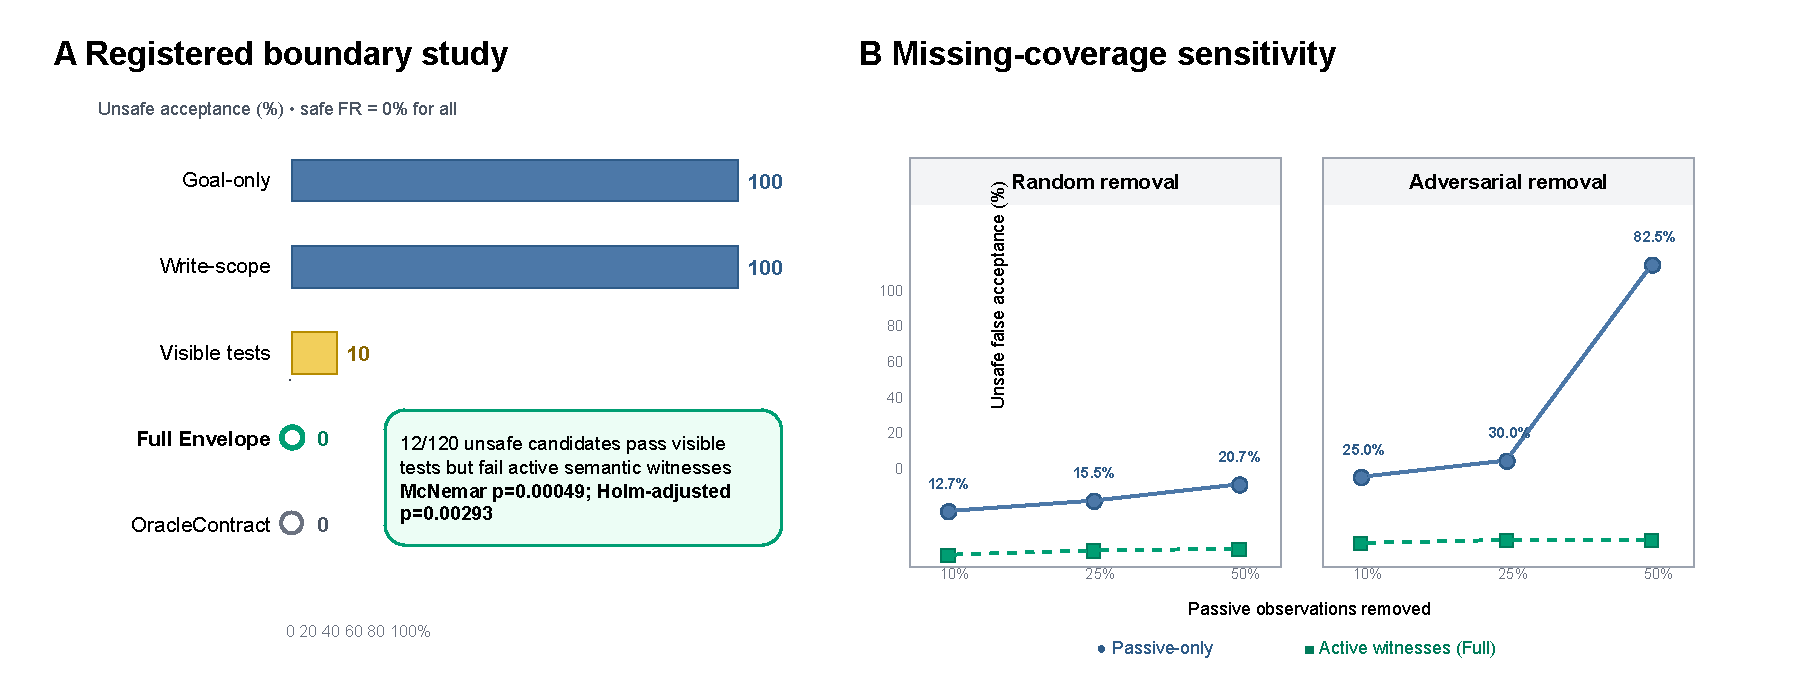
\includegraphics[width=0.98\textwidth]{figures/external_evidence.pdf}
  \caption{Registered public-corpus evidence.  (A) Full$_R$ closes 12 unsafe
  acceptances left by visible tests without rejecting registered-safe
  alternatives.  (B) active witnesses substantially reduce sensitivity to
  missing passive observations; all values are means over 20 replicates.
  Active witnesses are finite, not a completeness theorem, but remain at or
  below 5.0\% mean unsafe acceptance under every tested removal condition.}
  \label{fig:external-evidence}
\end{figure*}

\subsection{RQ3: separately specified models are complementary}

The registered oracle and Full$_R$ share a finite multi-vendor attribute
adapter.  To probe complementarity, we separately run Batfish queries outside
Full$_R$'s acceptance logic:
\texttt{searchRoutePolicies}/\texttt{compareRoutePolicies} over the frozen
candidates and additionally track metric and origin type.  Symbolic comparison
is applicable to 233/253 candidates and materializes 557 equivalence classes.
Twelve registered-safe candidates also change metric 200$\rightarrow$0 and
origin IGP$\rightarrow$EGP while changing authorized local preference;
Batfish conversely misses ten registered collateral cases.  Thus
Full$_R$=OracleContract establishes within-model consistency, not completeness.

One pair makes the gap concrete.  In Junos \texttt{09bea0}, a target term
changes local preference 200$\rightarrow$250 but also metric
200$\rightarrow$0 and origin IGP$\rightarrow$EGP, fields exposed only by the
Batfish audit.  In Arista \texttt{1dab61}, a shared action tags non-target
\texttt{10.100.0.0/16}; the registered frame rejects it, while the
target-scoped Batfish query does not classify it as unauthorized.  Neither
model subsumes the other.

Table~\ref{tab:cross-model} reports an exploratory audit on 162 jointly
applicable goal candidates, labeling a candidate unsafe if either model exposes
unauthorized behavior.  Full$_R$ and Batfish accept 12/119 and 10/119 unsafe,
respectively; their fail-closed conjunction (Full$_U$) accepts none and retains
all 43 cross-model-safe implementations.  Defined after the audit exposed the
gap, this union is not pooled with confirmation; it shows how explicit
obligations and provenance expose non-overlapping blind spots.

\begin{table}[t]
\caption{Exploratory cross-model audit on jointly applicable goal candidates.}
\label{tab:cross-model}
\centering
\footnotesize
\setlength{\tabcolsep}{3.6pt}
\begin{tabular}{lrrrr}
\toprule
Boundary & Unsafe acc. & FA & Safe rej. & FR \\
\midrule
Full$_R$ only & 12/119 & 10.1\% & 0/43 & 0\% \\
Batfish only & 10/119 & 8.4\% & 0/43 & 0\% \\
\textbf{Full$_U$ (AND)} & \textbf{0/119} & \textbf{0\%} & \textbf{0/43} & \textbf{0\%} \\
\bottomrule
\end{tabular}
\end{table}

\subsection{RQ4: end-to-end agent behavior}

\subsubsection{Agent128 safety and availability}

Table~\ref{tab:agent128} separates verified completion (VC),
goal-achieving collateral release (CR), failed-intent release (FI), terminal
transaction failure (TF), successful reject-to-safe repair, and attempt
exhaustion.  Direct and RAG release syntactic submissions, including non-goal
candidates.  Goal and write-scope release 61 and 59 collateral changes;
VerifierLoop reduces CR to five.  OracleContract and Full$_R$ release none in
the registered model; Full$_R$ repairs 16 first candidates and completes 49/128.

\begin{table}[t]
\caption{Agent128 end-to-end outcomes ($n=128$).}
\label{tab:agent128}
\centering
\scriptsize
\setlength{\tabcolsep}{2.5pt}
\begin{tabular}{lrrrrrr}
\toprule
Method & VC & CR & FI & TF & Repair & Exh. \\
\midrule
Direct replay & 33 & 56 & 39 & 0 & 0 & 0 \\
RAG one-shot & 16 & 48 & 63 & 1 & 0 & 0 \\
Goal-only & 43 & 61 & 0 & 0 & 10 & 24 \\
Write-scope & 39 & 59 & 0 & 0 & 6 & 30 \\
VerifierLoop & 40 & 5 & 0 & 0 & 7 & 83 \\
OracleContract & 45 & 0 & 0 & 0 & 12 & 83 \\
\textbf{Full$_R$} & \textbf{49} & \textbf{0} & \textbf{0} & \textbf{0} & \textbf{16} & \textbf{79} \\
\bottomrule
\end{tabular}
\end{table}

This is not ``safety for free.''  Full$_R$ fails closed in 79 events: 47 end
with semantic collateral and 32 still miss the target after five submissions.
Its higher VC than OracleContract is not attributed to the boundary because
revision calls are separate model samples after the paired first candidate.
The causal claim is confined to first-candidate acceptance; revision outcomes
measure operational behavior.

\textit{Post-freeze engineering analysis.}  Using the 79 exhaustions for
development, execution evidence and actionable transaction errors raise replay
to 128/128 without changing Full$_R$ acceptance.  Batfish then exposes 33
semantic failures and seven \na; frozen feedback repairs 32/33, so the
fail-closed union completes 120/128.  Agent128 uses 1,416 calls/6.40M tokens and
this replay adds 104 calls/1.04M tokens.  A label-independent 32-case holdout
completes 31/32 (one \na), with no measured unsafe release.  These results are
developmental, not confirmatory.

\subsubsection{Prior-workflow adaptations}

We adapt four workflows to the common task: the
classify--translate--generate--verify pipeline of
LLM-NetCFG~\cite{lira2024llmnetcfg}; INTA's fragment, retrieval, and refinement
stages~\cite{wei2025inta}; the verifier-guided prompt loop of CoSynth/Verified
Prompt Programming (CoSynth/VPP)~\cite{mondal2023router}; and the
inspect/edit/verify/rollback/submit agentic-repair loop
~\cite{asadli2026agentic} on Cornetto's public artifacts
~\cite{protogeros2026cornetto}.  They retain each paper's principal stages but
neither reproduce its native task nor rank the published systems.

We freshly select 48 public configurations, all file-disjoint and 46/48
topology-disjoint from controller development.  An excluded eight-case pilot
precedes the frozen 40-case split.  Arms share the model, temperature, baseline,
parsed context, transactions, 12-call/40k-token ceiling, and a sealed outcome
oracle consulted only after execution.  Only \system constructs active
witnesses; no arm sees a reference patch or oracle feedback.

Table~\ref{tab:external-methods} uses frozen Full$_R$; substituting Full$_U$,
defined only after RQ3 exposed a model gap, would make an exploratory repair
appear confirmatory.  Its results remain separate above.  VC is target-achieving
and oracle-safe, Unsafe is any released oracle-unsafe candidate, and Calls is
the per-case median.

\begin{table}[t]
\caption{Confirmatory common-task adaptations ($n=40$).}
\label{tab:external-methods}
\centering
\scriptsize
\setlength{\tabcolsep}{2.5pt}
\begin{tabular}{lrrrr}
\toprule
Method (adapted) & VC & Unsafe & Exh. & Calls \\
\midrule
LLM-NetCFG & 3 & 28 & 9 & 2.0 \\
INTA & 2 & 4 & 34 & 7.0 \\
CoSynth/VPP & 0 & 12 & 28 & 8.0 \\
Cornetto/Agentic & 18 & 10 & 12 & 9.0 \\
\textbf{\system Full$_R$} & \textbf{35} & \textbf{0} & \textbf{5} & \textbf{3.5} \\
\bottomrule
\end{tabular}
\end{table}

Against Cornetto/Agentic, \system reduces unsafe release by 25 points
(Holm $p=0.00391$; bootstrap 95\% CI 12.5--37.5) and raises VC by 42.5 points
($p=0.000221$; CI 25--60).  Unsafe reductions are Holm-significant against
LLM-NetCFG and CoSynth/VPP, but not INTA ($p=0.125$); the zero-unsafe Wilson
upper bound is 8.76\%.

\system completes 3/3 community, 4/4 legacy, 22/25 ordered-policy, and 6/8
shared-prefix cases with no measured unsafe release, using 171 calls versus
Cornetto/Agentic's 348.  These outcomes are specific to the common task and do
not rank the native systems.

In a paired trace, target \texttt{10.200.5.0/24} shares a list with three
non-target prefixes.  LLM-NetCFG and CoSynth/VPP release a shared-term edit
that changes all four preferences.  \system reports only the three observed
100$\rightarrow$150 deltas; the LLM's second attempt independently creates a
target-exclusive list and passes.  Feedback never names that list or command.

Of five \system exhaustions, three miss the target, one has a stale anchor, and
one retains shared-prefix collateral; all fail closed.  Pinned
Cornetto code and LLM-NetCFG artifacts guide their adaptations (no unlicensed
code copied); INTA and CoSynth/VPP are paper-faithful reimplementations because
no usable repository was available.  The manifest records provenance.

\subsection{RQ5: applicability and scale}

Batfish parses 234/253 candidates; 19 are \na, and a hard gate rejects three of
58 registered-safe candidates.  Symbolic comparison has 20/253 \na, never
promoted to PASS.  Single-process compiler time is 9.81~s at 100k FECs (100
objects), 25.83~s at 500 devices/100k FECs, and 90.92~s at the coupled
10k-object/100k-FEC point (42.63~MiB peak), excluding Batfish.  Agent128 LLM
latency P50/P95 is 2.07/3.55~s; Full$_R$ uses 343 calls and 1.54M tokens (12.0k
per case), excluding backend compute and price.  Rela/Kathara are not in these
scale counts.  The runner records backend attempts but does not aggregate
heterogeneous-container wall-clock, so LLM latency is not an end-to-end proxy.

\section{Discussion and Limitations}

\textbf{Conceptual role.}  \system separates implementation freedom from
release authority: the agent may invent any patch, while a pre-candidate
contract bounds its covered effects.  This matters most for shared objects,
ordered fall-through, and latent FECs.  The ablation supports the semantic frame
and active witnesses; this pool does not establish the independent necessity of
dependency and footprint guards.

\textbf{What the evidence supports.}  The frozen public-corpus study supports
contract compilation within the registered model: Full$_R$ matches the manual
OracleContract and closes collateral left by visible verification.  The
common-task study supports safer release and higher completion under its shared
protocol, not native-system superiority.  Batfish exposes metric/origin gaps
that Full$_R$ misses but misses registered community collateral.  It is
complementary, not ground truth; zero unsafe-release counts mean \emph{none
measured under the stated evidence model}.

\textbf{Where the claim stops.}  Only covered, applicable, verified behavior is
evidence of preservation; known \na and unmodeled dimensions are not.  Full$_U$
closes measured jointly applicable gaps, not unknown ones.  Normalization is a
trusted bottleneck.  Generated intents, a routing-policy subset, author-built
adaptations, limited public sources, and one endpoint constrain external
validity.  The endpoint limits repair availability and candidate diversity,
not deterministic acceptance over frozen candidates; the routing-policy subset
bounds semantic generality.

\textbf{Deployment.}  Fail-closed uncertainty costs availability: registered
Full$_R$ completes 49/128 and exhausts 79 cases.  Later recovery and holdout
results remain developmental.  Deployment requires a fresh snapshot,
invalidation on concurrent change, staging, rollback, and telemetry; a current
search anchor does not imply control-plane freshness.  Reported LLM cost
excludes backend compute.

\section{Related Work}

Recent LLM-based networking systems span benchmarking, generation, translation,
interaction, and repair.  NetConfEval benchmarks LLM configuration capability
under task-specific validation; it does not derive an intent-relative
preservation boundary~\cite{wang2024netconfeval}.  LLM-NetCFG maps
natural-language intent to configurations, while INTA translates fragments
across vendors with retrieval and staged verification
~\cite{lira2024llmnetcfg,wei2025inta}.  Accessible control and Clarify emphasize
interaction and ambiguity resolution~\cite{lin2025accessible,mondal2025clarify}.
AgentSpec enforces user-authored runtime rules across domains
~\cite{wang2025agentspec}; it does not derive network-semantic authority from a
Day-2 intent and pre-state.  Closest to our
repair loop, CoSynth/VPP couples an LLM with verifiers and turns localized
failures of supplied specifications into actionable regeneration feedback
~\cite{mondal2023router}.  Cornetto provides diverse configuration faults, and
agentic repair dynamically retrieves context, edits, verifies stated
properties, and rolls back regressions
~\cite{protogeros2026cornetto,asadli2026agentic}.
\system addresses the prior acceptance question: before any candidate, it
derives from the change intent and pre-state both the permitted target delta and
default-preserved non-target relations and reports frozen-boundary violations.

Classical verification systems establish complementary semantic facts.  Header
Space Analysis, VeriFlow, and APKeep verify forwarding invariants~\cite{kazemian2012hsa,
khurshid2013veriflow,zhang2020apkeep}; Batfish, Minesweeper, and Plankton model
configuration and control-plane semantics~\cite{fogel2015batfish,
beckett2017minesweeper,prabhu2020plankton,brown2023batfish}.  DNA and Rela make
pre/post change relations explicit~\cite{zhang2022dna,xu2024rela}.  Rela
compiles a supplied relational specification and two snapshots into an
automata-based check; it does not decide which unmentioned behaviors a Day-2
intent authorizes.  \system derives those obligations and routes supported path
and policy checks to Rela or Batfish; the Envelope determines which facts
acceptance requires.

Coverage and specification-mining systems address a different lifecycle point.
NetCov attributes a test suite's coverage to configuration lines and helps operators add tests
~\cite{xu2023netcov}.  \system uses a different unit and time: before a single
change, missing semantic classes trigger boundary/equivalence witnesses whose
non-target behavior enters the frozen contract.  Config2Spec, SelfStarter, and
MeshAgent infer network-wide invariants, templates, or latent requirements from
configuration corpora~\cite{birkner2020config2spec,kakarla2020templates,
zhou2025meshagent}.  An Envelope is instead intent-relative and ephemeral: it
states what one candidate may change and exposes what its finite evidence does
not cover.

Trusted synthesis systems instead choose an implementation for a supplied
specification.  NetComplete, NEAt, Snowcap, and Aura use trusted solvers to
synthesize configurations, repairs, or updates satisfying a
given specification~\cite{elhassany2018netcomplete,zhou2018neat,
schneider2021snowcap,ramanathan2023aura}.  Their trusted mechanism chooses an
implementation.  \system leaves object reuse, placement, and commands to an
untrusted LLM, then accepts any implementation satisfying a patch-independent,
pre-frozen boundary rather than a reference patch.

\section{Conclusion}

\system separates implementation freedom from release authority: before the LLM
authors a patch, an intent-derived Envelope freezes obligations without
prescribing an expected patch.  The contribution is not another verifier, but
the contract that determines what heterogeneous verifiers must establish for
release.  In 40 disjoint changes, \system completes 35 with no measured unsafe
release; the strongest adapted prior workflow completes 18 and releases ten
unsafe changes.  Making authority, coverage, \na, and residual uncertainty
explicit turns a verifier pass into an auditable, model-relative release
decision.

\bibliographystyle{IEEEtran}
\bibliography{references}

\end{document}
